% Tree

\documentclass{standalone}

%maths
\usepackage{tikz}
\usepackage{scalerel}
\usepackage{pict2e}
\usepackage{tkz-euclide}
\usetikzlibrary{calc}
\usetikzlibrary{patterns,arrows.meta}
\usetikzlibrary{shadows}
\usetikzlibrary{external}

%pgfplot

\usepackage{pgfplots}
\pgfplotsset{compat=newest}
\usepgfplotslibrary{statistics}
\usepgfplotslibrary{fillbetween}

%colours
\usepackage{xcolor}

\usepackage{nicefrac}



\begin{document}

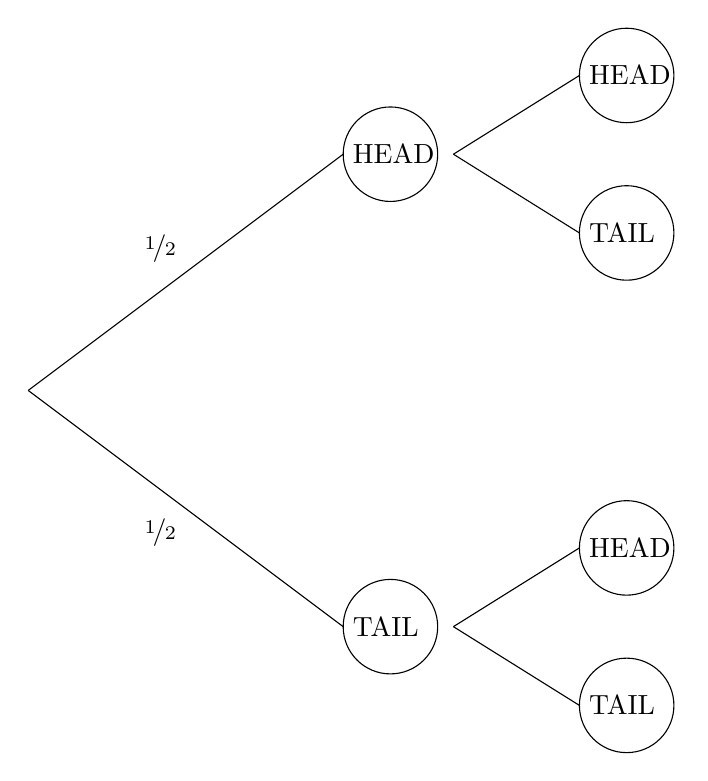
\begin{tikzpicture}[scale = 2]


\coordinate(o) at (0,0);
\coordinate[label = right : HEAD](a) at (2,1.5);
\coordinate[label = right : TAIL] (b) at (2,-1.5);

\draw (o) -- (a) node[midway, above left]{$\nicefrac{1}{2}$};
\draw (o) -- (b) node[midway, below  left]{$\nicefrac{1}{2}$};

\coordinate [label = right: HEAD] (a1) at (3.5, 2);
\coordinate [label = right : TAIL] (a2) at (3.5, 1);


\coordinate [label = right: HEAD] (b1) at (3.5, -1);
\coordinate [label = right : TAIL] (b2) at (3.5, -2);


\draw (2.7,1.5) -- (a1);
\draw (2.7,1.5) -- (a2);

\draw (2.7,-1.5) -- (b1);
\draw (2.7,-1.5) -- (b2);

\draw (2.3, 1.5) circle [radius=0.3];
\draw (2.3, -1.5) circle [radius=0.3];
\draw (3.8, 2) circle [radius=0.3];
\draw (3.8, 1) circle [radius=0.3];
\draw (3.8, -1) circle [radius=0.3];
\draw (3.8, -2) circle [radius=0.3];




\end{tikzpicture}


\end{document}